\documentclass[11pt]{article}
\usepackage{amsmath}
\usepackage{amsthm}
\usepackage{graphicx}
\usepackage{hyperref}
\usepackage[utf8]{inputenc}
\usepackage{enumitem}
\usepackage{cancel}
\usepackage{latexsym}
\usepackage{amsfonts}
\usepackage{bussproofs}
\usepackage{tikz}
\nocite{*}

\newcommand{\A}{{\mathbb~A}}
\newcommand{\Evp}{{Ev (\bar{p})}}
\newcommand{\CTLf}{{CTL$^f$ }}
\newcommand{\X}{{\mathbf{X}}}
\newcommand{\F}{{\mathbf{F}}}
\newcommand{\orr}{{\vee}}
\newcommand{\andd}{{\wedge}}
\newcommand{\phii}{{\varphi}}
\newcommand{\G}{{\mathbf{G}}}
\newcommand{\dia}{{\diamondsuit}}
\usepackage[a4paper, total={6in, 9in}]{geometry}

\bibliographystyle{plain}


\title{MPRI Internship Report}
\author{Anatole Leterrier, supervised by Sam van Gool, IRIF}
\date{2022--07--2022}

\newtheorem*{definition}{Definition}

\begin{document}

\maketitle

\section*{}

\subsection*{General context}
Temporal logics are at the heart of the domain of program verification.
When reasoning about the behavior of a program, not only do we want 
to know which properties are true at the present, but we also need 
to be able to predict what will happen at some time in the future.
Along with the usual propositional language, these logics include
temporal operators like `next', `future', or others characterizing
the existence of a branch in a tree where a property is true
infinitely often.
As  with any logic, we would like to prove that the chosen syntactical
axiomatization engenders the whole set of semantically valid properties.
Such proofs often use techniques from Stone duality, Büchi automata and
tableaux, as I also do in this report.

\subsection*{Problem studied}
The completeness of Linear Temporal Logic (LTL), the most straighforward
of those logics, is a very well known result. It usually boils down
to the Satisfiability problem, that is, to deciding whether a formula
has a semantical model. Other, more complex temporal logics exist, such 
as \CTLf(Computational Tree Logic with fairness constraints). Silvio
Ghilardi and Sam van Gool proved the completeness of the latter logics.
In their proof, Stone duality makes for an impressive tool in order to
reason over axioms as properties of relations over Kripke structures. 

While satisfiability of a formula can be known for those logics, computing
an actual model is another problem. We would like to find an algorithm
which contructs one such model, if possible. Apart from the practical
benefits of such an algorithm, this research provides global information 
about how temporal logics work. This is not obvious, as
the proofs we mentioned are not constructive: they make use of Stone 
ultrafilters in infinite algebras, which are sets of formulas which 
generally cannot be characterized by a finite subset.

\subsection*{Contributions}
This report presents the following contributions:

- A detailed comparison of the several ways LTL completeness
(\emph{ie.} the SAT problem) is handled
in the literature. SAT has 
multiple approaches using Büchi automata which recognize particular
LTL formulas, so I helped clarify the link between states
of the automata associated with the formula,
and atoms in a particular algebra generated by the formula.
This allows to stay closer to the essential notion of Stone duality.

- I have re-explained~\cite{GhivG17}
in terms of Stone duality extended to `LTL-algebras'. Other approches 
to SAT make use of tableaux, structures which are both algorithmic-friendly,
and very close to the research of models for formulas. 

- I implemented Reynolds' tableaux
algorithm for solving SAT in LTL~\cite{ReyLTL}, which is a most recent work in this vein.
Along with the binary answer to the SAT problem, it provides a model when
it can.

- I have studied `{\CTLf}algebras' in order to characterize
{\CTLf}formulas by atoms. This is a first step into making the proof in~\cite{GhivG16} constructive.



\subsection*{Arguments supporting their validity}
/////



\subsection*{Summary and future work}
/////
\newpage  

\section{Introduction}
This section contains a few preliminaries, to make the reader more familiar with the
content at discuss in this report. Beyond the definitions given in the section, we expect
a few basic notions of finite automata, Boolean algebra and  logics from the reader.
\subsection{LTL (Linear Temporal Logic)}
In the most general setting, logics are sets of structural rules, which are intended to
formalize an ensemble of true properties of some system. Although the origins of logics can 
be dated back to Aristotle's syllogisms, they found new life with the advent of computer 
science, as a tool for verification of systems, and automation of proofs. It is hard
for a computer to prove a theorem on its own, using the human way of thinking; however,
bringing a theory down to a finite set of rules, the search for proofs falls into the 
understanding of computer systems. Throughout this paper, we will speak of \emph{syntax} when
considering the formal system of the logic: axioms and inference rules. On the other hand,
\emph{semantics} define the actual meaning of formulas; they tell whether we should consider a
formula to be satisfied in some system we chose.

The simplest logic is the classical propositional calculus, defined for instance in~\cite{PropLog}. 
The set of formulas of propositional logic over a set of Boolean variables 
$\{p_1,\ldots,p_n\}$ can be restated as the \emph{Free Boolean Algebra}\cite{GehvG22}$(A,\orr,\neg,\bot)$
over this set,
where the classical, well-known implications and equivalences over Boolean algebras hold. From now
on, we will prefer condensing syntax of logics as a compact restatement of the set of rules
in terms of Boolean Algebra. This will allow us to escape long lists of rules, focusing on the
structure of our logics.

Temporal logics were first introduced by A. Pnueli in 1977, and can be
viewed as an enrichment of propositional calculus with time constraints. We begin with the simplest
such logic:

\begin{definition}\label{LTL}
    \emph{Linear Temporal Logic} (LTL) consists of the language of propositional logic, along with
    operators defined on every formula:
    \begin{itemize}
        \item[-] $\dia$ is the \emph{Next} operator. Syntactically, it is defined as a Boolean 
            endomorphism over the Boolean algebra $(A,\orr,\neg,\bot)$. Semantically, if $\phii$ is 
            a formula of LTL, $\dia\phii$ is 
            satisfied in a state if $\phii$ is satisfied in the next state. We will precise what this
            `next state' is in the context of our work.
        \item[-] $\F$ is the \emph{Future} operator, which also stands for `finally'.
            For every formula $\phii$ in LTL, $\F\phii$ is defined as the least pre-fixpoint of the
            function $x\mapsto \phii\orr\dia\F x$. Semantically, $\F\phii$ is satisfied whenever there
            exists a state in the future (or in the present) where $\phii$ holds. Algrebraically,
            $\F$ is a \emph{unary modal operator}, which also is \emph{join-preserving}:
            $\F(\phii\orr\psi)=\F\phii\orr\F\psi$.
        \item[-]$\G$ \emph{(Globally)} is a syntactical shortcut for $\neg\F\neg$, which means that $\G\phii$ is true 
            only when
            $\phii$ holds forever from the current state on. By symmetry, it is a meet-preserving,
            unary modal operator: $\G(\phii\andd\psi)=\G\phii\andd\G\psi$.
    \end{itemize}
\end{definition}
Note that the definition of LTL usually includes operator $\mathbf{U}$ (\emph{until}), which we will not
discuss here.
Another remark: while it holds for every $\phii$ that $\phii\orr\dia\F\phii\leq\F\phii$, we actually
get an equality for this last inequality. Indeed, $\dia(\dia\F\phii\orr\phii)=\dia\phii\orr\dia\dia\F\phii$,
which is below $\dia\F\phii\orr\dia\F\phii$, by definition of $\F$ and by monotonicity of $\dia$. This
is itself below $\dia\F\phii\orr\phii$. Now, by minimality in the definition of $\F$, it holds that
$\F\phii\leq\F(\dia\F\phii\orr\phii)\leq\dia\F\phii\orr\phii$, which proves that the first inequality
exactly is an equality.

\begin{definition}\label{infinite word}
    Now, we precise the semantical meaning of `next' and `future' operators.
    An \emph{infinite word} over some set $S$ is a sequence $(s_n)$ of 
    elements (or \emph{nodes}) in $S$. 
    Finally, for a finite set $\bar{p}$ of
    variables, define a \emph{$\bar{p}$-coloring} $\sigma : S \to \mathcal{P}(\bar{p})$.

    We can define the forcing relation $\models$ between nodes in $S$ and formulas $\phii$ with 
    variables in $\bar{p}$, by induction on $\phii$:
    \begin{itemize}
        \setlength\itemsep{0em}
        \item[-] $s\not\models \bot$;
        \item[-] $s \models p$ if $p \in \sigma(s)$;
        \item[-] $s \models \neg\phii$ if not $s \models \phii$;
        \item[-] $s \models \phii \vee \psi$ if $s\models \phii$ or if $s\models \psi$;
        \item[-] $s\models \dia\phii$ if the unique successor of $s$, $s'$ is such that
             $s'\models \phii$;
        \item[-] $s\models \F\phii$ if there exists $n\geq 0$, such that in the unique path 
            $s_0,s_1\ldots s_n$ ($s_0=s$), $s_n\models\phii$;      
    \end{itemize}

\end{definition}

Also, note that $s\models \G\phii$ if and only if in the unique path $s=s_0,s_1\ldots s_n$, we have
$s_n\models\phii$ for every $n\geq 0$.


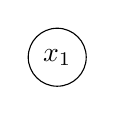
\begin{tikzpicture}[main/.style = {draw, circle}] 
    \node[main] (1) {$x_1$}; 
\end{tikzpicture}


\subsection{Fair CTL (Computational Tree Logic)}
CTL is a very common temporal logic, operating over infinite trees instead of infinite words.
It consists of operators such as AX (`all successors verify\ldots') and EG
(`there exists a branch where globally \ldots holds'). However, in~\cite{GhivG16}, an evolved variant named
\CTLf~was introduced, allowing to add fairness constraints on branches. Let us define precisely
what it means.

\subsubsection*{Syntax of fair CTL}\label{subsec:syntax_CTLf}

\begin{definition}\label{CTLf_formulas}
    Let $\bar{p}= \{p_1,\ldots,p_n \}$ be a finite set of propositional variables. We define inductively 
    a \emph{$CTL^{f}$-formula} $\varphi$ to be of the shape:
    \begin{itemize}
        \setlength\itemsep{0em}
        \item[-] $\bot$
        \item[-] $p \in \bar{p}$
        \item[-] $\neg \varphi$
        \item[-] $\varphi \vee \psi$
        \item[-] $\dia \varphi$
        \item[-] $EU(\varphi,\psi)$
        \item[-] $EG(\varphi,\psi)$ 
    \end{itemize}
    For convenience, we then also define the De Morgan duals of our binary operations, respectively $\wedge$ for $\vee$; $AR$ for $EU$; $AF$ for $EG$. For the unary operator, we set $\Box \varphi = \neg \dia(\neg \varphi)$; Finally, we set $\top$ to be the negation of $\bot$, naturally.
\end{definition}


\begin{definition}\label{quasi_eq_CTLf}
    We define the \emph{quasi-equational theory $CTL^{f}$} by requiring the formulas to satisfy the following axioms:
    \begin{enumerate}
        \setlength\itemsep{0em}
        \item Boolean algebra axioms for $\vee,\neg,\bot$;
        \item Unary operator $\dia$ preserves finite joins, including the empty joint $\bot$, making $CTL^f$ into a modal logic (\cite{GehvG22});
        \item $\dia \top = \top$
        \item Binary operators $EU$ and $EG$ satisfy the following \emph{fixpoint axioms} for all $a,b,c$:
        \begin{itemize}
            \item[-] $a \vee (b \wedge \dia EU(a,b)) \leq EU(a,b)$
            \item[-] $a \vee (b \wedge \dia c) \leq c \implies EU(a,b) \leq c$ 
            \item[-] $EG(a,b)\leq a\wedge \dia EU(b\wedge EG(a,b),a)$
            \item[-] $c\leq a\wedge \dia EU(b\wedge c,a) \implies c \leq EG(a,b)$
        \end{itemize}
        In other words, $EU(a,b)$ is the \emph{least pre-fixpoint} of the function $x \mapsto a \vee (b \wedge \dia x)$.
        And $EG(a,b)$ is the \emph{greatest post-fixpoint} of the function $x \mapsto a\wedge \dia EU(b\wedge x,a)$.
    \end{enumerate}
\end{definition}

Importantly, we remark that for all $a,b$, $AR(a,b)$ is the greatest post-fixpoint of $x \mapsto a \wedge (b \vee \Box x)$, while $AF(a,b)$ is the least pre-fixpoint of $x \mapsto a \vee \Box AR(b\vee c,a)$.

What is called a \emph{quasi-equational theory} corresponds to what we expect of a syntax. That is, there are \emph{equations} (equalities) which correspond to axioms of a deduction system, like: \AxiomC{}\UnaryInfC{$\top\vdash\dia\top$} \[\DisplayProof\]
But there also are \emph{quasi-equations} (implications) which translate to deduction rules: \AxiomC{$c\vdash a\wedge \dia EU(b\wedge c,a)$}\UnaryInfC{$c \vdash EG(a,b)$}\[\DisplayProof\]
However, we rarely (or never) use the rules properly speaking, but we define a structure which embodies those properties and use operations on it. This is a step in advance towards semantics, in some sense.
\begin{definition}\label{CTLf-algebra}
    Given what is said above, we can deduce the definition of a \emph{$CTL^f$-algebra}, which is a tuple $\A=(A,\bot,\neg,\vee,\dia,EU,EG)$ which verifies every axiom of $CTL^f$ quasi-equational theory.
\end{definition}

Also, the way EU and EG formulas are defined reminds the fixpoint operators of the \emph{$\mu$-calculus}. For example, for every $a,b$, $EU(a,b)$ could have been defined as $\mu x.(a \vee (b \wedge \dia x))$, the least fixpoint of this monotone function (it is enough to say the least \emph{pre-fixpoint})\cite{Santo08}. As for EG, it is a greatest \emph{(post-)} fixpoint, so it could have been defined with a $\nu$ operator, where $\nu f = \neg\mu(\neg f) $. More precisely: \[EG(a,b)=\nu.y(a\wedge\dia\mu.x((b\wedge y)\vee(a\wedge\dia x))).\] This makes apparent a nesting of a $\nu$ and a $\mu$ operator. This is what makes the logic hard to simplify, compared to LTL which only contains one such fixpoint operator.  
\begin{definition}\label{interp_form_algebra}
    For any finite set of propositional variables $\bar{p}$ and any $CTL^f$-algebra $\A$, we can define a \emph{valuation} $V:\bar{p}\to A$. Then any $CTL^f$-formula $\varphi$ with variables in $\bar{p}$ can be interpreted as a term in $A$ (the \emph{interpretation} of $\varphi$ under $V$, $\varphi^A(V)$).

    Then, we can say the equality $\varphi(\bar{p})=\psi(\bar{p})$ is \emph{valid} if it interprets to $\top$ under every valuation to every $\A$.

    $\varphi$ and $\psi $ are said to be \emph{equivalent} if the equation $\varphi = \psi$ is valid. $\varphi$ is called a \emph{tautology} if it is equivalent to $\top$, and is said to be \emph{consistent} if it is not equivalent to $\bot$.

    Finally, we say $\varphi$ \emph{entails} $\psi$ if $\neg \varphi \vee \psi$ is a tautology, which we will note $\varphi \vdash \psi$ or $\varphi \leq \psi$.
\end{definition}

\subsubsection*{Semantics of fair CTL}\label{subsec:sem_CTLf}
\begin{definition}\label{forcing_rel_CTLf}
    We first define the notion of \emph{transition system}, ie.\ a pair $(S,R)$, where $S$ is a set, and $R$ a binary relation on $S$. Then, a \emph{$R$-path} is a (possibly infinite) sequence of nodes in $S$ such that $s_i R s_{i+1}$ for all $i$. Finally, for a finite set $\bar{p}$ of variables, define a \emph{$\bar{p}$-coloring} $\sigma : S \to \mathcal{P}(\bar{p})$.

    We can define the forcing relation $\models$ between nodes in $S$ and formulas $\varphi$ with variables in $\bar{p}$, by induction on $\varphi$:
    \begin{itemize}
        \setlength\itemsep{0em}
        \item[-] $s\not\models \bot$;
        \item[-] $s \models p$ if $p \in \sigma(s)$;
        \item[-] $s \models \neg\varphi$ if not $s \models \varphi$;
        \item[-] $s \models \varphi \vee \psi$ if $s\models \varphi$ or if $s\models \psi$;
        \item[-] $s\models \dia\varphi$ if there exists $s'$ such that $sRs'$ and $s'\models \varphi$;
        \item[-] $s\models EU(\varphi,\psi)$ if there exists $n\geq 0$ and a path $s_0Rs_1R\ldots Rs_n$ ($s_0=s$) such that $s_k\models\psi$ for every $k<n$ and $s_n\models\varphi$;
        \item[-] $s\models EG(\varphi,\psi)$ if there exists an infinite path $s_0Rs_1R\ldots $ ($s_0=s$) such that $s_k\models\varphi$ for every $k$ and $s_j\models\psi$ infinitely often on the path.       
    \end{itemize}

\end{definition}

Remark that as a consequence, $s\models\Box\varphi$ if and only if for every successor $s'$ of $s$ by $R$, $s'\models\varphi$ holds.
Also, $s\models AR(\varphi,\psi)$ if and only if for every $n\geq 0$ and every path $s=s_0Rs_1R\ldots Rs_n$, either $s_k\models\psi$ for some $k<n$, or $s_n\models\varphi$.

Similarly, $s\models AF(\varphi,\psi)$ if and only if for all infinite paths ${(s)}_k$ starting from $s_0$, if $s_j\not\models\psi$ infinitely often, then $s_k\models\varphi$ for some $k$.

Also, as a convention, we will consider the transition systems to be \emph{serial}, ie.~that every node has a successor. Syntactically, this is represented by the axiom $\dia\top = \top$.

\section{Satisfiability of LTL: a comparative analysis}

\section{Reynolds' SAT Solver for LTL: an implementation}
\subsection{Reynolds' tableaux algorithm for LTL}
- Why this algo?

- Description of the algo
\subsection{An implementation in Ocaml}
\subsubsection*{Why Ocaml?}

- Describe my program: how it works (main fct)

- How it computes models (remains to be done)


\section{Towards a constructive proof for completeness of fair CTL}





\bibliography{bibli}
\end{document}